\section*{PROPOSED HYBRID MODEL FOR ROLL DAMPING}\label{sec:hybrid_damping_model}

%\subsection*{\textbf{Ikeda's damping components}} \label{subsec:hybrid_ikeda}

When the damping predicted with Ikeda's method was compared with corresponding model test it was found that the results were in poor agreement for the zero speed case but quite good results at speed. This was pointing towards the eddy damping being incorrect in the current
implementation of Ikeda's method. A thorough investigation of the eddy damping prediction was therefore conducted in the next section.

\textbf{\textit{Eddy damping}} The eddy damping is due to eddies generated around the ship hull during the roll motion. Strong eddies occures at sharp edges in the geometry. Below is an illustration of how the eddy damping changes with bilge radius to beam ratio as predicted with the current implementation of the method. It seems that the damping approaches zero very fast as the bilge radius increase. So having just a small rounding of the bilge, compared to a square section, will have a great impact on the eddy roll damping.

    \begin{figure}[H]
        \begin{center}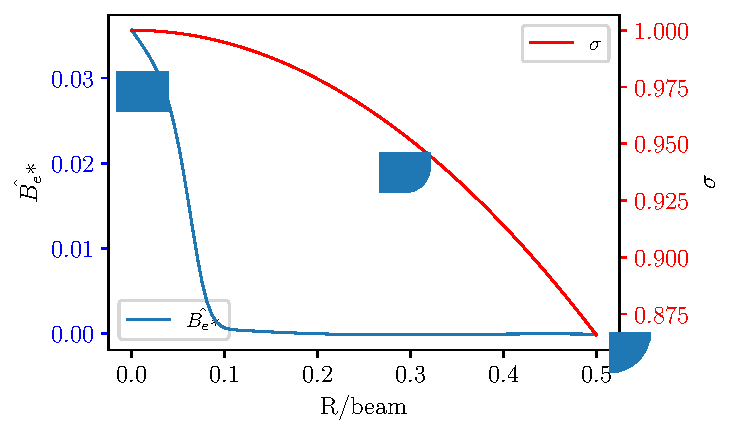
\includegraphics[width = 0.5\textwidth]{figures/eddy_sigma.pdf}\end{center}
        \vspace{-1cm}
        \caption{Eddy sigma}
        \label{fig:eddy_sigma}
    \end{figure}
    
Ikeda made experiements on a number of two-dimensional cylinders with various sections \cite{7505983/4AFVVGNT}. Ikeda found that the eddy damping per unit length of these sections can be expressed as: 

    
\begin{equation}
B'_{E0} = \frac{4 C_{r} T_{s}^{4} \omega \phi_{a} \rho}{3 \pi}
\label{eq:eddy_section}
\end{equation}

    
The total eddy damping can be obtained as an integral over the sections along the ship hull:
 
    
\begin{equation}
B_{E0} = \int\limits_{AP}^{FP} B'_{E0}\, dx
\label{eq:equation}
\end{equation}

    
It can be seen from the section damping (eq. \ref{eq:eddy_section}) above that the eddy damping increases linearly with both roll amplitude and frequency, and that it will go to zero for small amplitudes and frequencies, which means that it is only included in the quadratic damping term ($B_2$). Ikeda expressed the
$C_r$ coefficient to be entirely depending on the hull form. Ikeda developed a regression formula for $C_r$ based on his experiments, which is used in the prediction method. The authors of this paper have tried to implement this method according to the description in the original paper \cite{7505983/4AFVVGNT} but have failed to reproduce the
results from Ikeda's experiments exactly. Other resources such as \cite{7505983/FB64RGPF} and \cite{7505983/KAKIM2E2} have also been used without success.


\subsection*{\textbf{Hybrid model for damping}} \label{subsec:hybrid_formula}
Instead, a new regression for $C_r$ was made on the experimental
results from \cite{7505983/4AFVVGNT}. The experimental results were
collected by the authors using manual digitalization
\cite{7505983/RXYIE6UW}.

Where $OG/d=0$ for all sections. For the Series60 sections (G-K) the bilge radius $R_b$ was estimated using the following estimation, proposed by the authors:
 
\begin{equation}
R_{b} = \frac{\sqrt{B_{s} T_{s} \left(1 - \sigma\right)}}{\sqrt{1 - \frac{\pi}{4}}}
\label{eq:equation}
\end{equation}

    
The nondimensional damping is expressed in \cite{7505983/4AFVVGNT} using an asterisk, or star symbol (*). The reason seems to be that Ikeda wanted to signal that this damping only has the quadratic part of the
damping. This stared damping is defined as:
 
\begin{equation}
B_{E0 HAT} = \frac{8 B_{E star hat}}{3 \pi}
\label{eq:equation}
\end{equation}

    
$\hat{B_E}^*$ and $(B_W+B_F)^*$ are the experimental values taken from \cite{7505983/4AFVVGNT}. Which add up to the total damping: 

$\hat{B^*} = \hat{B^*_E} + (B_W+B_F)^*$
 
\begin{equation}
B_{E0 HAT} = \frac{8 B_{E star hat}}{3 \pi}
\label{eq:equation}
\end{equation}

    
And the $C_r$ was calculated from the experiments as:

    
\begin{equation}
C_{r} = \frac{3 \pi B_{E0 HAT} B_{s} T_{s} beam^{2} \sigma}{4 T^{4} \omega_{hat} \phi_{a}}
\label{eq:equation}
\end{equation}

    

Instead of trying to invent a complicated mathematical expression for the $C_r$ regression a simple decision tree model was instead fitted to the $C_r$ data from Ikeda's experiments. The fitted decision tree is illustrated in the figure below:

    \begin{figure}
        \begin{center}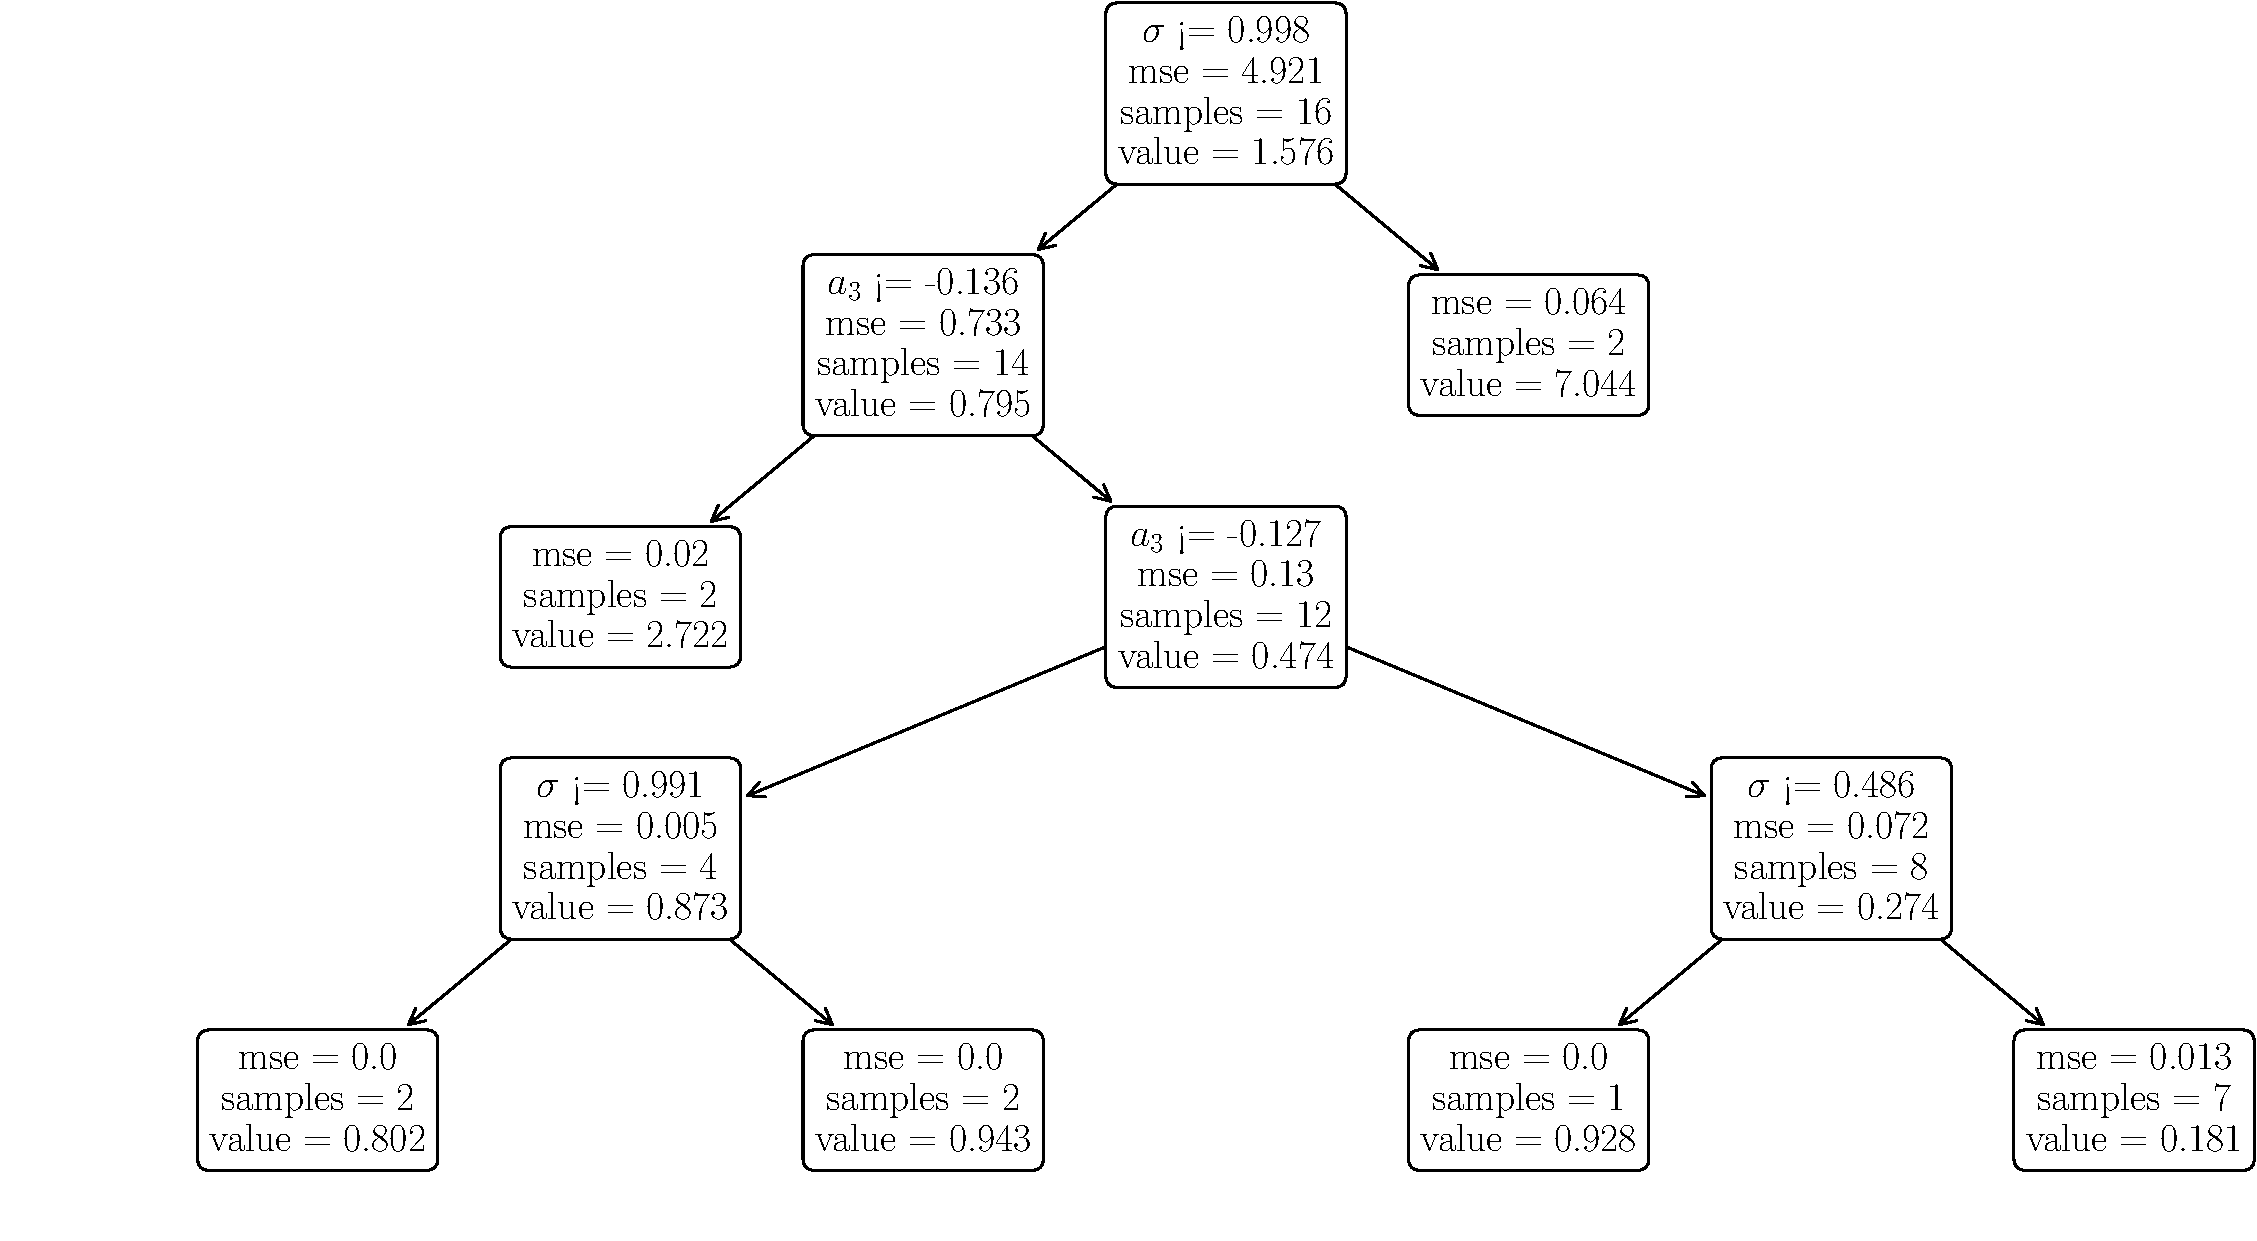
\includegraphics[width = 0.4\textwidth]{figures/decision_tree.pdf}\end{center}
        \vspace{-0.5cm}
        \caption{Decision tree}
        \label{fig:decision_tree}
    \end{figure}
    
Even thoug this tree is very simple it has very good accuracy in reproducing the results from Ikedas experiments ($r^2=0.996)$.

\subsection*{\textbf{Wave making damping by FNPF}} \label{subsec:hybrid_FNPF}
Wave damping was obtained using PIT on roll decay
simulation using the fully nonlinear potential flow method. This method is characterized by the application of the complete dynamic and kinematic free surface boundary conditions on the instantaneous free surface as well as the body-exact approach where the instantaneous wetted body surface is considered in the boundary value problem for the velocity potential, i.e. no linearizations are made to the governing equations of the potential flow problem.

The method used in this study employs a boundary element method (BEM) \cite{7505983/FD4N3DW2} to solve the boundary value problem for the velocity potential. The free surface boundary conditions and the motions of the floating
body introduce time dependency to the boundary value problem. The BEM is coupled with the mixed Eulerian-Lagrangian method (MEL) \cite{7505983/ZKB494GT} which is used for the evolution of free surface.
A fourth-order Adams-Bashforth-Moulton time integral scheme is then used to evolve free surface and the rigid-body body motions in time.

The benefit with the FNPF method is the lack of linearizations to the free surface potential flow where all interactions between the undisturbed incident flow and surface piercing body is captured implicitly in the total velocity potential, including inviscid (wave) damping due to radiation and diffraction. The downside is the larger
computational cost compared to many other potential flow based methods due to the fact that a boundary value problem for the velocity potential must be solved at least once every time step, depending on the specifics
of the time integral scheme. However, FNPF methods are still typically less computationally demanding than for example URANS methods, making them attractive choices for seakeeping problems.